\documentclass[a4paper,12pt]{report}
\usepackage[dvips]{color}
\usepackage{lscape}
\usepackage{color}
\usepackage{times}
\usepackage{url}
\usepackage{rotating}
\usepackage[pdfborder={0 0 0}]{hyperref}
\usepackage{breakurl}  %DS added Oct9. Needs to be after hyperref
\usepackage{parskip}
\usepackage[margin=2cm]{geometry}
\usepackage[margin=2cm]{caption}
\usepackage{etoolbox}
\usepackage{longtable}
\usepackage{nicefrac}
\patchcmd{\quote}{\rightmargin}{\leftmargin 1em \rightmargin}{}{}

\usepackage{ulem}   % added by dave to allow strike-out below
\newcommand{\QUERY}[1]{{\color{red}{#1}}}
\newcommand{\NEW}[1]{{\color{blue}{#1}}}
\newcommand{\DEL}[1]{{\color{red}{\sout{#1}}}}
\newcommand{\COMMENT}[1]{{\color{magenta}{#1}}}

\usepackage{fancyhdr}
\usepackage{times}
\setlength{\headheight}{15pt}
 
\pagestyle{fancyplain}
\renewcommand{\chaptermark}[1]{\markboth{#1}{}}
 
\lhead{\fancyplain{}{\thepage}}
\chead{}
\rhead{\fancyplain{}{\textit{\leftmark}}}
\lfoot{}
\cfoot{}
\rfoot{}



%\hypersetup{
%    pdfborder={0 0 0}    % fits the width of the page to the window
%}


%\usepackage[Sonny]{fncychap}
%\usepackage[Bjarne]{fncychap}
%\usepackage[Lenny]{fncychap}
%\usepackage[Glenn]{fncychap}
%\newcommand{\ug}{$\mu g m^{-3}$}
%ST
\newcommand{\degrees}{\ensuremath{^\circ}}
 \newcommand{\ug}{\ensuremath{\mu \mbox{g m}^{-3}}\,}
\newcommand{\tug}{$\nicefrac{\mu g}{m^{3}}$}
\newcommand{\ugN}{\ensuremath{\mu \mbox{g(N) m}^{-3}}}
\newcommand{\tugN}{$\nicefrac{\mu g(N)}{ m^{3}}$}
\newcommand{\ugS}{\ensuremath{\mu \mbox{g(S) m}^{-3}}} 
\newcommand{\tugS}{$\nicefrac{\mu g(S)}{m^{-3}}$}

\newcommand{\mgSl}{\ensuremath{\mbox{mg(S)l}^{-1}}} 
\newcommand{\tmgSl}{$\nicefrac{mg(S)}{l}$} 
\newcommand{\mgNl}{\ensuremath{\mbox{mg(N)l}^{-1}}}
\newcommand{\tmgNl}{$\nicefrac{mg(N)}{l}$} 
\newcommand{\mgl}{\ensuremath{\mbox{mg l}^{-1}}}
\newcommand{\tmgl}{$\nicefrac{mg}{l}$} 
\newcommand{\mgSm}{\ensuremath{\mbox{mg(S)m}^{-2}}}  
\newcommand{\tmgSm}{$\nicefrac{mg(S)}{m^{2}}$} 
\newcommand{\mgNm}{\ensuremath{\mbox{mg(N)m}^{-2}}}
\newcommand{\tmgNm}{$\nicefrac{mg(N)}{m^{2}}$}
\newcommand{\tmgm}{$\nicefrac{mg}{m^{2}}$}  

%%% I tried using \bv to start a small-tex verbatim section and
%%% \ev to end this. However, it seems that \end{verbatim} needs to
%%% to be written explicitly, so I use \ev now to end the small-text.
%%% Place directly after \end{verbatim}.

%% \newcommand{\bv}{\begin{small}\begin{verbatim}}
%% \newcommand{\ev}{\end{small}}

\newcommand{\Par}{{\bf Par\_ml}}
\newcommand{\MyOutputs}{{\bf My\_Outputs\_ml}}

\begin{document}% \sloppy
%\begin{landscape}

\title{{\huge The EMEP/MSC-W Model }\\
{\Large unofficial User's Guide}}

\date{October 2015}
\maketitle

\tableofcontents
\setcounter{page}{0}

\chapter{Welcome to EMEP }

This guide gives a brief documentation of the EMEP/MSC-W model
version rv4.8. 
It is intended primarily as a guide on how to run the model, and
to help users wishing to understand or change 
the model in terms of domains, outputs, chemistry, etc.


The main documentation for the EMEP/MSC-W model is an article pulished 
in Atmospheric Chemistry and Physics in 2012. 
This article will be referred to as Simpson et al. (2012) in
this manual. 


\begin{itemize}
\item
Simpson, D., Benedictow, A., Berge, H., Bergstr\"om, R., Emberson, L.D., Fagerli, H., Flechard, C.R., Hayman, G.D., Gauss, M., Jonson, J.E., Jenkin, M.W., Ny\'iri, \'A, Richter, C., Semeena, V.S, Tsyro, S., Tuovinen, J.-P., Valdebenito, \'A., and Wind, P.:
The EMEP MSC-W chemical transport model – technical description.  
Atmospheric Chemistry and Physics, 12, 7825-7865, 2012. \\
\url{http://www.atmos-chem-phys.net/12/7825/2012/acp-12-7825-2012.html}
\end{itemize}


The model source code is available from the EMEP/MSC-W Open Source website:\\ 
\url{https://wiki.met.no/emep/page1/emepmscw_opensource}

\newpage

\section{Licenses and Caveats}

The EMEP code is provided under the GNU General Public License version 3
(\url{http://fsf.org} and/or
\url{http://www.gnu.org/copyleft/gpl.html}).

Each code module is prefaced with something like:\\
\bigskip

\begin{quote}
\begin{footnotesize}
\begin{verbatim}
! <EXAMPLE_CODE.f90 - A component of the EMEP MSC-W  Eulerian
!          Chemical transport Model>
!*******************************************************************!
!*
!*  Copyright (C) 2007-2016 met.no
!*
!*  Contact information:
!*  Norwegian Meteorological Institute
!*  Box 43 Blindern
!*  0313 OSLO
!*  NORWAY
!*  email: emep.mscw@met.no
!*
!*    This program is free software: you can redistribute it and/or modify
!*    it under the terms of the GNU General Public License as published by
!*    the Free Software Foundation, either version 3 of the License, or
!*    (at your option) any later version.
!*
!*    This program is distributed in the hope that it will be useful,
!*    but WITHOUT ANY WARRANTY; without even the implied warranty of
!*    MERCHANTABILITY or FITNESS FOR A PARTICULAR PURPOSE.  See the
!*    GNU General Public License for more details.
!*
!*    You should have received a copy of the GNU General Public License
!*    along with this program.  If not, see <http://www.gnu.org/licenses/>.
!*******************************************************************!
\end{verbatim}
\end{footnotesize}
\end{quote}

And a copy of the license file, {\bf gpl.txt}, is provided with the
model code source files.

\noindent It is important to note that the code is provided ``as it is'', 
and EMEP/MSC-W has very limited resources with which to support
usage of the code. 

%% To help users an {\bf EMEP Forum} is available from the
%% EMEP/MSC-W Open Source website in section ``Users'': ``EMEP Forum''. 
%% Support to the user community will develop here with your contribution. 
%% Please let us know what your needs for information are 
%% (e-mail: emep.mscw@met.no).

\newpage

\section{Computer Information}
\label{sec:compinf}

To compile the EMEP/MSC-W model you need:\\

\textbf{Fortran 95 compiler}

\textbf{NetCDF Library ($>$4.1.3)}

\textbf{MPI Library ($>$1.0)}\\

It is necessary to compile with double precision reals (8 bytes
reals). The program has been used on computers ranging from a Linux laptop to supercomputers 
(Itanium2 cluster, Intel Xeon cluster, Cray XT4, IBM power5+). It is compatible with all 
compilers tested so far:  Intel, PGI, gfortran, XL fortran. A Makefile is included,  
the path to netcdf (INCL and LLIB) have to be adapted to your machine, and the fortran 
compiler (F90) and flags (F90FLAGS) to the compiler you are using.



The code has been tested with 1 to 1024 CPUs, and scales well (for large grids).  If only one 
CPU is used 1-2 GB memory is required. If more than one,
for example 64 CPUs are used, 200 MB of memory per CPU is enough (in
the case of a 132 X 159 grid size). For runs on more than 32 CPUs, a fast interconnect is 
recommended (infiniband for example), for smaller runs, gigabit ethernet is sufficient. 
It takes $\sim$ 5 hrs on 64*Xeon X5355 (2.66GHz) for 1 year simulation.

When downloading input data in order to do a ``base run'' please make
sure that there are 35 Gb disc space available, especially due to
large meteorology input files. The model can be run for shorter periods, users 
can download meteorology for only the period they are interested in, pluss one day. 
 

\section{Getting Started}


It is recommended to read all the chapters of this EMEP/MSC-W model
User Guide before you start downloading anything from the EMEP/MSC-W Open
Source website.

%% Please register as an EMEP User on the {\bf EMEP Forum}
%% (EMEP/MSC-W Open Source website under ``Users'' section: ``EMEP Forum'')
%% before you start downloading the EMEP/MSC-W model code and/or input
%% data. This will give you access to further communication with the
%% developing team and to the section on ``Questions and Answers''. 


This is what you need to do before you can do a ``base run'' with the 
EMEP/MSC-W model:

\begin{itemize}
%\item Register as an EMEP User
\item Read the EMEP/MSC-W model User Guide
\item
Download input data (description in Chapter~\ref{ch:InputFiles} and
data available from the EMEP/MSC-W Open Source website under ``Download''
section: ``Input Data'')
\item
Download the EMEP/MSC-W model source code (description in 
section~\ref{sec:ModelCode} and the files are available from the EMEP/MSC-W 
Open Source website under ``Download'' section: ``Model Code'')
\item
Follow the instructions for ``Submitting a Run'' description in
Chapter~\ref{ch:SubmitARun}.
\item
Download some model results for comparison, description in
Chapter~\ref{ch:output} and the files are available from the EMEP/MSC-W 
Open Source website under ``Download'' section: ``Model Results''. 
%NEWTOOLS:
% \item
% If wanted, download some helper programmes to read site and sonde outputs, 
% see sections~\ref{sec:tools},\ref{sec:sitesonde}.
% The files are available from the EMEP
% Open Source website under ``Download'' section: ``Tools''.


\end{itemize}

\section{Model code}
\label{sec:ModelCode}

The EMEP/MSC-W model code version rv.4.8 are archived as a tar file. 
The tar file is called ``EMEP\_MSC-W\_model.rv4.8.OpenSource.tar.gz'' and 
is downloadable from the EMEP/MSC-W Open Source website.

Once this file is untarred all model files needed for a model run will be 
found under the directory \\ {\bf EMEP\_MSC-W\_model.rv4.8.OpenSource/code/} 
where the model source code, makefiles, and a copy of the license file are 
stored. An overview is given in Table~\ref{Tab:modelfiles}

\begin{table}[h]
\begin{center}
\caption{Contents of ``EMEP\_MSC-W\_model.rv4.8.OpenSource.tar'' file
   \label{Tab:modelfiles}}
\begin{tabular}{ll}
& \\
\hline
Type      & Filename          \\
\hline
& \\
{\bf Model code directory} & EMEP\_MSC-W\_model.rv4.8.OpenSource/code \\ 
\hline
modules files & *.f90 \\
include files & *.inc \\
namelist & config\_emep.nml \\
makefiles & Makefile and Makefile.SRCS \\
dependency file &  dependencies\\
a copy of the license & gpl.txt \\
\hline
\end{tabular}
\end{center}
\end{table}

In addition there is a run script called ``modrun.sh'', which will be placed 
in the \\{\bf EMEP\_MSC-W\_model.rv4.8.OpenSource/}  directory. The run 
script, ``modrun.sh'', can easily be modified to work on your computer system. 
This script is described in detail in Chapter \ref{ch:SubmitARun}. 
 
%NEWTOOLS
% \section{Helper tools}
% \label{sec:tools}
% ????
% For users interested in reading the ascii site and sonde specific outputs,
% two help programmes (Rd\_sites.f90, Rd\_sondes.f90) are provided, 
% in the \\{\bf EMEP\_Unified\_model.OpenSource2012/tools}  directory. These
% programmes are readily compiled with e.g. gfortran, and can be run without
% arguments to obtain usage instructions. See section~\ref{sec:sitesonde}
% for more details.


\section{Model grid}
\label{sec:ModelGrid}

The current EMEP model version, and the provided gridded input data,
have a horizontal resolution of 50$\times$50 km$^2$ (at 60$^\circ$N)
and are defined on a
polar stereographic projection with 20 sigma levels vertically. 
The model is very flexible with regard to the horizontal
resolution, in that it readily makes use of 
meteorological data provided with the model. The vertical
resolution is currently still restricted to the fixed 20 layer
system. The physical
description is given in detail in Chapter 2 of the EMEP Status Report
1/2003 Part I (Simpson {\sl et al.}, 2003).

In 2008 the EMEP domain was extended eastwards in order to include the 
EECCA countries in the EMEP model grid, see Figure \ref{fig:EECCA}. To distinguish the new grid from the old EMEP 
grid, the new grid is called EECCA in this text and in the config\_emep.nml.

\begin{figure}[ht]
 \centering
%DS 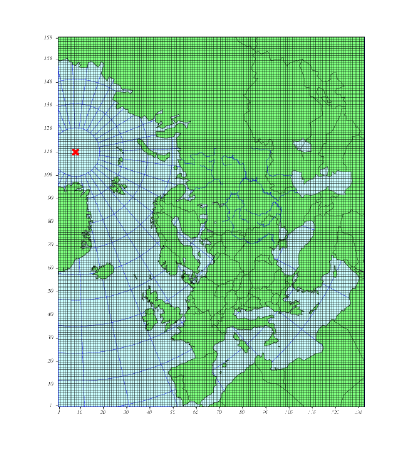
\includegraphics[scale=0.7]{EECCA}
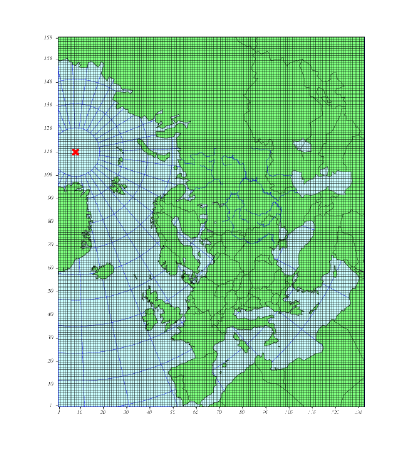
\includegraphics[scale=1.1]{EECCA}
\caption{The extended EMEP grid covering EECCA area with
132$\times$159 gridpoints on 50$\times$50 km$^2$ resolution defined on
a polar stereographic
projection.}\label{fig:EECCA}
\end{figure}

\chapter{Input files}
\label{ch:InputFiles}

This chapter provides an overview on the necessary input files to run the 
EMEP/MSC-W model. A complete set of input files is provided in the EMEP/MSC-W 
Open Source web page to allow model runs for the meteorological year 2013. 

The input files are zipped in 13 different files. There are 12 zipped files 
for the meteorology, one for each month, called meteo2013MM.tar.bz2 (where MM 
is the month). 
The last file for December also include a met file for January 1$^{st}$ 2014. 
The last zipped input file (called other\_input\_files.tar.bz2) contains all 
other input files needed for running the EMEP/MSC-W model, except the aircraft emissions,
AircraftEmis\_FL.nc, and the forest fire emissions, FINN\_ForestFireEmis\_2013.nc. See sections~\ref{emisair} and \ref{emisff} for details about these emissions data.

After unzipping all the meteo tar files, the meteorology are placed under a
catalogue called {\bf EMEP\-\_MSC-W\_model.OpenSource2015/}. The met/
catalogue should be moved over to current version of model, for rv4.8:
{\bf EMEP\_MSC-W\_model.rv4.8.OpenSource}. 
So now there will be two directories under 
{\bf EMEP\_MSC-W\_model.rv4.8.OpenSource}. 
All meteorology are placed under /met, and the rest of the input files under 
/input. 
All files, both meteorological and the other input files, are described in 
this chapter.

{\bf IMPORTANT:} The input data available in the EMEP/MSC-W Open Source Web
site should be appropriately acknowledged when used for model runs.
If nothing else is specified according to references further in this
chapter, please acknowledge EMEP/MSC-W in any use of these data.

\begin{table}
\caption[List of input data files]{List of input data files.
Note: YYYY: year, MM: month, DD: day, SS: seasons, POLL: pollutant
type (NH$_3$, CO, NO$_x$, SO$_x$, NMVOC,
PM$_{2.5}$ and PM$_{co}$). 
\label{Tab:inputdata}}
\begin{center}
\begin{small}
% \hspace{-1cm}
\begin{tabular}{lll}
\hline
{\bf Data} &  {\bf Name} & {\bf Format}\\
{\bf Meteorology data} & met/&  \\
Meteorology  &  meteoYYYYMMDD.nc \quad (365+1 files) & netCDF\\
& & \\
{\bf Other Input files} & input/ &\\
Global Ozone & GLOBAL\_O3.nc & netCDF\\
New Global Ozone & Logan\_P.nc & netCDF $^*$$^*$\\
BVOC emissions & EMEP\_EuroBVOC.nc & netCDF\\
Landuse & LanduseGLC.nc and Landuse\_PS\_5km\_LC.nc  & netCDF\\
Degree-day factor & DegreeDayFactors.nc &  netCDF\\
N depositions & annualNdep.nc  & netCDF\\
Road dust &  RoadMap.nc and AVG\_SMI\_2005\_2010.nc& netCDF$\dagger$ \\
Aircraft emissions & AircraftEmis\_FL.nc & netCDF$\dagger$ \\
Surface Pressure & SurfacePressure.nc & netCDF$\dagger$ \\
Forest Fire & FINN\_ForestFireEmis\_YYYY.nc & netCDF$\dagger$ \\
& & \\
Dust files  &Soil\_Tegen.nc  & netCDF$\dagger$\\
 & SoilTypes\_IFS.nc & netCDF$\dagger$\\
% Landuse & Inputs.Landuse & ASCII$^*$\\
% Land/Sea mask & landsea\_mask.dat & ASCII\\
Emissions & emislist.POLL  \quad ({\footnotesize 7 files, EMEP 50km PS grid}) & ASCII\\
 & Emis\_TNO7.nc \quad ({\footnotesize regional, 0.125$\times$0.0625 lon-lat})& netCDF$\dagger$\\
 & Emis\_GLOB\_05.nc \quad ({\footnotesize global, 0.5$\times$0.5 lon-lat})& netCDF$\dagger$\\
Vertical level distribution & Vertical\_levels.txt & ASCII\\
Time factors for monthly emissions& MonthlyFac.POLL  \quad (7 files) & ASCII\\
Time factors for daily emissions &  DailyFac.POLL  \quad (7 files) & ASCII\\
Time factors for hourly emissions & HOURLY-FACS  & ASCII$^*$\\
Emission heights & EmisHeights.txt & ASCII$^*$\\
Natural SO$_2$ & natso2MM.dat  \quad (12 files) & ASCII\\
Volcanoes & columnsource\_emission.csv & ASCII$^*$\\
	  & columnsource\_location.csv& ASCII$^*$ \\ 
Lightning emissions & lightningMM.dat  \quad (12 files) & ASCII$^*$\\
Emissions speciation & emissplit.defaults.POLL & ASCII$^*$\\
                     & emissplit.specials.POLL & ASCII$^{*,\dagger}$\\
Emission factors for scenario runs & femis.dat & ASCII\\
Photo-dissociation rates & jclearSS.dat \quad (4 files) & ASCII\\
 & jcl1kmSS.dat \quad (4 files) + jcl1.jun & ASCII\\
 & jcl3kmSS.dat \quad (4 files) + jcl3.jun & ASCII\\
Landuse definitions & Inputs\_LandDefs.csv & ASCII$^*$\\
Stomatal conductance & Inputs\_DO3SE.csv & ASCII$^*$\\
Sites locations for surface output & sites.dat & ASCII$^*$\\
Sondes locations for vertical output & sondes.dat & ASCII$^*$\\
\hline
\end{tabular}\\

\vspace{0.5cm}
Notes: $\dagger$ - optional (in most cases); 
$^*$ means ASCII files with header.
$^*$$^*$ New O3 boundary condition data in 30 levels.  Can be used with 'NewLogan=.true.' in 'BoundaryConditions\_ml.f90'.
\end{small}
\end{center}

\end{table}

\newpage


\section{NetCDF files}



\subsection{Meteorology}
The daily meteorological input data (``meteoYYYYMMDD.nc'', where YYYY is year, MM is month 
and DD is day) used for the EMEP/MSC-W Model are based on
forecast experiment runs with the Integrated Forecast System (IFS), a global
operational forecasting model from the European Centre for Medium-Range
Weather Forecasts (ECMWF).

The IFS forecasts has been run by MSC-W as
independent experiments on the HPCs at ECMWF with special requests on
some output parameters. The meteorological fields are retrieved on a
0.1$^{\circ}\times$0.1$^{\circ}$ longitude latitude coordinates and interpolated to
50$\times$50 km$^2$ polar-stereographic grid projection. Vertically, the fields
on 60 eta levels from the IFS model are interpolated onto the 37 EMEP sigma
levels.  The meteorology is prepared into 37 sigma levels since the model is 
under test for a finer vertical resolution.  But the Opensource code is released
with 20 sigma levels and to make the model read the meteorology properly, 
a description of the 20 vertical sigma levels is needed.  This is provided in 
an ascii file called 'Vertical\_levels.txt' together with the other\_input data. 
The version of the IFS model used for preparing these fields,
Cycle 38r2, is documented in \url{http://www.ecmwf.int/research/ifsdocs/index.html}. Previous years are based on Cycle 36r1 with a resolution of 0.2$^{\circ}\times$0.2$^{\circ}$ on a spherical grid. 
Meteorological fields currently used for EMEP/MSC-W Model runs are given in
Table~\ref{Tab:metinput}. Some verification and description of these
meteorological fields are given in Chapter 2 of the EMEP Status Report
1/2015.

{\bf Acknowledgement:} ECMWF, met.no

\newpage
\begin{table}[h!]
\caption{Input meteorological data used in the EMEP/MSC-W Model
   \label{Tab:metinput}}
\begin{center}
\begin{tabular}{p{6cm}lll}
\hline
Parameter      & Unit & Description          \\
\hline
\multicolumn{3}{l}{3D fields - for 37 $\sigma$ levels} \\
$u,v$  &  m/s     & Horizontal wind velocity components   \\
$q$    &  $\nicefrac{kg}{kg}$   & Specific humidity           \\
%$\dot{\sigma}$ & s$^{-1}$ & Vertical wind in $\sigma$ coordinates \\
$\theta$       & K  & Potential temperature \\
$CW$             & $\nicefrac{kg}{kg}$ & Cloud water          \\
$CL$             & \% & 3D Cloud cover            \\
$cnvuf$          & $\nicefrac{kg}{sm^2}$ & Convective updraft flux \\
$cnvdf$          & $\nicefrac{kg}{sm^2}$ & Convective downdraft flux \\
$PR$             & mm & Precipitation         \\
\hline
\multicolumn{3}{l}{2D fields - for Surface} \\
$PS$             & hPa & Surface pressure                     \\
$T2$          & K  & Temperature at 2m height               \\
$Rh2$             & \% & Relative humidity at 2m height \\
SH              &  $\nicefrac{W}{m^{2}}$ & Surface flux of sensible heat \\
LH             & $\nicefrac{W}{m^{2}}$ & Surface flux of latent heat \\
$\tau$         & $\nicefrac{N}{m^{2}}$ & Surface stress               \\
SST            & K & Sea surface temperature \\
SWC            & $\nicefrac{m^{3}}{m^{3}}$ & Soil water content      \\
%DSWC           & m$^3$/m$^{3}$ & Deep soil water content$^\ast$   \\
lspr             & m & Large scale precipitation \\
cpr              & m & Convective precipitation \\
sdepth         & m & Snow depth \\
ice            & \% & Fraction of ice \\  
$SMI1$           &    & Soil moisture index level 1 \\
$SMI3$           &    & Soil moisture index level 3 \\
u10/v10        & m/s  & wind at 10 m height \\
\hline
\end{tabular}\\
%Notes: $\ast$ not yet used
\end{center}
\end{table}

\subsection{Gridded emissions}
\label{emisnew}

Since 2015 different formats of gridded emissions can be used and
mixed (with some restrictions) under one common framework. The
different formats that are presently supported are: 
\begin{enumerate}
\item ``Old style'' ASCII emissions format. Total yearly emissions.

The gridded emission files contain 16 columns where the first column 
represents the country code
(\url{http://www.emep.int/grid/country_numbers.txt}), 
the second and the third columns are the `i' and `j' indices of the
EMEP grid, the fourth and fifth columns are the total emissions from
low and high sources, and the last 11 columns contain emissions from 
10 anthropogenic SNAP sectors.

The advantage of the ASCII emissions format, is that they are easy to
modify, and the interpretation of the numbers is straightforward. 
The main disadvantage of the ASCII emissions format, is that they are
only valid for one specific grid projection. Visualization of these
emissions, needs also some more efforts. 

\item Countrywise NetCDF emissions. Yearly totals.

Each country and sector has its own NetCDF field.

The main advantage of NetCDF emissions is that all the information
about the data (projection, units) is given in the same file. This
allows the code to reproject the emissions to any grid projection on
the fly. It is easy to visualize the emissions of one country with
simple tools, like ncview. The data is simple to interpret and it is
possible to add new countries to an existing file (with appropriate
tools). 

The disadvantage of countrywise NetCDF emissions, is that there are
quite a large number of fields, with most of the data being
zero. NetCDF will compress the data, but it will still take some time
for the model to read all the data. 
 
\item ``Fraction type'' NetCDF emissions. Yearly totals.

The total emissions are stored in one gridded map, and in addition
information about which country the emission belongs to. 

The main advantage of ``fraction type'' NetCDF emissions, is that they
will keep the grid flexibility, have a more compact form and be faster
to read in. 

The disadvantage is that the interpretation of the content of the
fields is more difficult and it is hard, for instance, to add a new
country to the file. Total emissions and coverage of countries can
easily be visualized, but not emissions from one single country. 



\begin{table}
\caption{Description of main fields for ``fraction type'' NetCDF Emissions}
\label{Tab:Emisdata}
\begin{center}
%\begin{small}
% \hspace{-1cm}
\begin{tabular}{lll}
\hline

{\bf Variable name } & {\bf Description}\\

Ncodes & Number of countries sharing the same grid cell\\
poll\_secNN & Pollutant from each sector \\
Codes & Country code number \\
fractions\_poll\_secNN & Fraction of emissions to assign to one country\\

\hline

\end{tabular}
\end{center}
%\end{small}
\end{table}





\item Monthly ``fraction type'' NetCDF emissions.

This is similar to the yearly ``fraction type'' NetCDF emissions, but
there are 12 monthly values for each field. This format cannot be
combined with other formats. 

\end{enumerate}

\subsubsection{Using and combining gridded Emissions}

These gridded emission files are controlled via the ``config\_emep.nml'' file.
Each file is assigned as one set of values for emis\_inputlist.
An ASCII emission file can be included for instance with the line:

\begin{quote} \begin{verbatim}
emis_inputlist(1)\%name = '/MyPathToEmissions/emislist.POLL',
\end{verbatim} \end{quote} 

``POLL'' is a keyword, which will be replaced by the model by all the emitted pollutants (according to the 
names defined in ``CM\_EmisFiles.inc'').

An additional NetCDF emission file can be included for instance with the line:
\begin{quote} \begin{verbatim}
emis_inputlist(2)\%name = '/MyPathToEmissions/Emis\_GLOB\_05.nc',
\end{verbatim} \end{quote} 

Now all emissions from both ASCII file and NetCDF file will be used. In practice some countries might be counted twice. Therefore some new data can be included in the ``emis\_inputlist'', to specify which countries to keep or to avoid. Example:

\begin{quote} \begin{verbatim}
emis_inputlist(1)\%incl(1:) = 'NO','SE','FI',
emis_inputlist(2)\%excl(1:) = 'NO','SE','FI',
\end{verbatim} \end{quote} 

Will include only 'NO','SE' and 'FI' from the first file (ASCII), and take all countries except 'NO','SE' and 'FI' from the second file (NetCDF).

Sets of countries can in principle be defined; for now only the set 'EUMACC2' is defined.

\subsection{Global Ozone}
Initial concentration of ozone are required in order to
initialize the model runs. Boundary conditions along the sides of the model
domain and at the top of the domain are then required as the model is
running.

The Logan\_P.nc file contains monthly averaged fields in netCDF format. 
The initial and background
concentrations are based on the Logan (1998) climatology. The Logan
climatology is scaled by Unimod according to the Mace Head measurements as
described in Simpson {\sl et al.} (2003). For a number of other species, 
background/initial conditions are set within the model using functions 
based on observations (Simpson {\sl et al.}, 2003 and Fagerli {\sl et al.}, 2004).

\subsection{BVOC emissions}
Biogenic emissions of isoprene and monoterpene are calculated in the
model as a function of temperature and solar radiation, using the landuse
datasets. The light and temperature depencies are similar to those
used in the original open source model, see 
Chapter 4.2 of the EMEP Status Report 1/2003 Part I (Simpson
{\sl et al.}, 2003).

Biogenic VOC emission potentials (i.e. rates at 30$^\circ$C and full sunlight)
are included for four different forest types in the netCDF file 
EMEP\_EuroBVOC.nc. These emission potentials have unit $\mu g/m^{2} /h$, and
refer to emissions per area of the appropriate forest category. In 
addition, default emission potentials are given for other
land-cover categories in the file Inputs\_LandDefs.csv. 
The underlying emission potentials, land-cover data bases, and model
coding have however changed substantially since model version v.2011-06. The new approach
is documented in Simpson {\sl et al.}, 2012.

\subsection{Landuse}

Landuse data are required for modeling boundary layer processes
(i.e. dry deposition, turbulent diffusion).
The EMEP/MSC-W model can accept landuse data from any
data set covering the whole of the domain, providing reasonable 
resolution of the vegetation categories. Gridded data sets providing
these landuse categories across the EMEP domain have been created
based on the data from the Stockholm Environment Institute at York 
(SEI-Y) and from the Coordinating Center for Effects (CCE). 
16 basic landuse classes have been identified for use in the
deposition module in the model, and three additional ``fake'' landuse
classes are used for providing results for integrated assessment
modeling and effects work.

There are two netcdf files included, one file ``Landuse\_PS\_5km\_LC.nc`'' on 5 km resolution over the EMEP domain, and a global ``LanduseGLC.nc''. The different landuse types are desribed in Simpson et al (2012). 

% There is a {\bf header} in the file that contains short abbreviations 
% for the different land cover
% types, e.g. CF for temperate/boreal coniferous forest. The landuse
% types are summarized in Table 5.1 in Chapter 5 of the EMEP Status
% Report 1/2003 Part I (Simpson {\sl et al.}, 2003).
% 
% The different landuse types are given as a percentage of area for each 
% EMEP grid cell in the {\bf ASCII file} ``Inputs.Landuse''. 

\subsection{Degree-day factor}
Domestic combustion which contribute to a large part of SNAP 2, varies on the daily 
mean temperature. The variation is based on the heating degree-day concept. These 
degree days are pre-calculated for each day and stored in the file DegreeDayFactors.nc. 
See Simpson et al. (2012) section 6.1.2. 


\subsection{NO$_x$ depositions}
Areas with high NO deposition loads have greater soil-NO emissions. To include this in 
the model, a netcdf file where pre-calculated N-depositions are included. The file made by 
the results from the EMEP/MSC-W model runs over a 5-year period. 


\subsection{Road Dust}
Road traffic produces dust. These emissions are handled in the EMEP/MSC-W model in the 
{\bf Emissions\_ml.f90} module. To include road dust, set USE\_ROADDUST = .true. in ``config\_emep.nml''. There are two files included in input data, RoadMap.nc and 
AVG\_SMI\_2005-2010.nc. RoadMap.nc include gridded roads and PM emissions over Europe, 
AVG\_SMI\_2005-2010.nc are global. 

\subsection{Aircraft emissions}
\label{emisair}

In the EMEP/MSC-W model aircraft emissions are 'OFF' by default. 
They can be switched 'ON' by setting USE\_AIRCRAFT\_EMIS = .true. in ``config\_emep.nml'' and download the data from \url{http://www.pa.op.dlr.de/quantify}.  
The EMEP model uses data provided by the EU-Framework Programme 6 Integrated 
Project QUANTIFY (\url{http://www.pa.op.dlr.de/quantify}). However, before using 
these data a protocol has to be signed, which is why the data file can not be provided 
directly on the EMEP/MSC-W Open Source website. If you want to use aircraft emissions go to 
\url{http://www.pa.op.dlr.de/quantify}, click on 'QUANTIFY emission inventories and scenarios', 
and then click on 'Register'. That page will provide information about the registration 
process and the protocol that has to be signed. Once you are registered, click 'Login' and 
provide user name and password. On the new page, search for 'Emissions for EMEP', which 
links directly to the Readme file and the emission data file in netCDF format. Download the 
emission data file and place it in the input folder.

\subsection{Surface Pressure}

If USE\_AIRCRAFT\_EMIS = .true. in { \bf config\_emep.nml,} then in addition to the Aircraft 
Emission file, there will be need for a SurfacePressure.nc file, which is already in the /input folder. 
The netCDF file consists of surface pressure fields for each of the months in 2008 called surface\_pressure, 
and one field for the whole year called surface\_pressure\_year. All fields are given in Pa. 

\subsection{Forest Fire}
\label{emisff}

Since model version rv3.9 (November 2011), daily emissions from forest and vegetation fires are taken from the “Fire INventory from NCAR version 1.0” (FINNv1,
Wiedinmyer et al. 2011). Data are available from 2005, with daily resolution, on a fine 1 km×1 km grid. We store these data on a slightly coarser grid (0.2$^\circ$×0.2$^\circ$) globally for access by the EMEP/MSC-W model. To include forest fire emissions set 
USE\_FOREST\_FIRES = .true. in ``config\_emep.nml'' and download the 
2012 GEOS-chem daily data \url{http://bai.acd.ucar.edu/Data/fire/}. The data needs to be stored with units mole/day in a netCDF file called FINN\_ForestFireEmis\_2013.nc 
compatible with the { \bf ForestFire\_ml.f90 } module. 

\subsection{Dust files}

The annual ascii data for sand and clay frations as well as the monthly data for boundary and initial conditions for dust from Sahara are replaced with a single netCDF file 'Soil\_Tegen.nc' since 2013.   This covers data for a global domain in 0.5$\times$0.5 degree resolution.  

The variables 'sand' and 'clay' gives the fraction (in \%)  
of sand an clay in the soil for each grid cell over land. 

%((The files are provided by 
%Maxilian Posch, Netherlands Environmental Assessment Agency, CCE, pers%onal communication?????.)) 


The files are used by the module {\bf DustProd\_ml.f90}, which calculates windblown dust 
emissions from soil erosion. Note that the parametrization is still in the development and 
testing phase, and is by default 'turned off'. To include it in the model calculations, set 
USE\_DUST = .true. in ``config\_emep.nml''.
The user is recommended to read carefully documentation and
comments in the module {\bf DustProd\_ml.f90}.

There is also a possibility to include boundary and initial conditions for dust from Sahara. 
The input file gives monthly dust mixing 
ratios (MM - month, e.g. 01, 02, 03,...) for fine and coarse dust from Sahara. The files are based on calculations 
from a global CTM at the University of Oslo for 2000. 
To include Saharan dust, set USE\_SAHARA = .true. in ``config\_emep.nml''.

Another source for dust is an arid surface. This is accountet for by soilmosture calculations in {\bf DustProd\_ml.f90 }. 
Together with Soil Water Index from the meteorology files and permanent wilting point (pwp) from SoilTypes\_IFS.nc. 
This file is global and netcdf. See Simpson et al. (2012) section 6.10.



\section{ASCII files}


% 
% 
% 
% \subsection{Land/Sea mask}
% This file, based on the meteorological model's roughness length, is used
% to assign a land/sea mask within the  EMEP/MSC-W model, since there is
% a need to modify the stability information for coastal grid cells
% (which contain land, but is not resolved by the NWP model supplying 
% meteorological data to the EMEP model). 
% 
% The gridded {\bf ASCII} file ``landsea\_mask.dat'' contains 3 columns. 
% The first two columns represent the `i' and `j' indices of the EECCA
% grid and the third column gives the class of the grid cell, where the 
% EMEP model use 0 for ocean, and $\geq$ 1 as land.



\subsection{Natural $SO_2$}
Natural $SO_2$ emissions (dimethylsulfide (DMS) from sea) are provided 
as monthly gridded files.  
The values are given at the surface in $\mu$g/m$^2$ for each grid cell in the domain. 

\subsection{Volcanoes}

Emissions from volcanic passive degassing of $SO_2$ are included for
the active Italian volcanoes, Etna and Stromboli, based upon the
officially submitted data.
To consider these volcanic emissions, we need to feed the locations
and heights of volcanoes into the model. The input file
"columnsource\_location.csv" contains the geographical coordinates
(latitudes and longitudes) and 
the heights (in meters) of the
included volcanoes, while "columnsource\_emission.csv" contains the
emission parameters.

Since 2010 the EMEP model has also been used to model the transport of
ash and $SO_2$ from volcanic eruptions. In addition to data for
passive degassing of $SO_2$, the above two input files also contain
locations and emission parameters for two recent eruptions of Icelandic
 volcanoes (Eyjafjallaj\"okull in 2010 and Grimsv\"otn in 2011). In
order to include emissions from these eruptions one needs to set
'USE\_ASH=T' (F by default) in ``config\_emep.nml''.


%% The input file ``VolcanoesLL.dat'' in {\bf ASCII} format contains the input data for the two active volcanoes
%%  Enta and Stromboli. The two first columns gives their latitudes and longitudes, their height as sigma level
%%  in column 3 and their emission in ktons per year in column 4. 

\subsection{Gridded emissions}

The official emission input for the EMEP/MSC-W model consists of
gridded 
annual national emissions based on emission data reported every year
to EMEP/MSC-W (until 2005) 
and to CEIP (from 2006) by each
participating country. 
More details about the emission input with references can be
found in Chapter 4 of the EMEP Status Report 1/2003 Part I 
(Simpson et al., 2003).

Since 2015 different formats of gridded emissions can be used and
mixed (with some restrictions) in the EMEP model under one common
framework. The new emission system is described in
section~\ref{emisnew}. Here we focus only on the "old style" ASCCI
emission format.  

Seven gridded emission input files (``emislist.poll'') are available
in  
{\bf ASCII} format for the following compounds: CO, NH$_{3}$,
NO$_{x}$, PM$_{2.5}$, PM$_{co}$, SO$_{x}$ and VOC.


The gridded ASCII emission files
contain 16 columns where the first column  
represents the country code
(\url{http://www.emep.int/grid/country_numbers.txt}), 
the second and the third columns are the `i' and `j' indices of the
EMEP grid, the fourth and fifth columns are the total emissions from
low and high sources, and the last 11 columns contain emissions from 
10 anthropogenic SNAP sectors 
(\url{http://reports.eea.eu.int/technical_report_2001_3/en}) and 1 
source-sector called``Other sources and sinks'', which include natural and
biogenic emission sources. The data are given with the unit: $Mg$.

{\bf Acknowledgement:} EMEP

\subsection{Time factors for emissions}

Monthly and daily time factors for emission of the 7 compounds 
(CO, NH$_{3}$, NO$_{x}$, PM$_{2.5}$, PM$_{co}$, SO$_{x}$ and VOC). 
There is one file available per compound in {\bf ASCII} format. 

The first two columns in the files represent the country code \\
(\url{http://www.emep.int/grid/country_numbers.txt}), the second column 
represents the sector (\url{http://webdab.emep.int/sectors.html}). In the monthly files, 
the 12 consecutive columns represent the time factors corresponding to 
the months of the year. In the daily files there are 7 consecutive columns representing 
the time factor for each day of the week. 

The file HOURLY-FACS 
includes factors for each of the eleven SNAP sectors for every hour (the columns) for 
each day of the week, see Simpson et al. (2012) section 6.1.2

% \COMMENT{I moved all emission-related factors here}

\subsection{Emission heights}
A vertical distribution for the elleven SNAP sectors are given in the file EmisHeights.txt. 
The file has seven vertical levels, over the collumns and the SNAP sectors given in the first row. 
Read more in Simpson et al. (2012) section 6.1.1.

\subsection{Emission factor for scenario runs}\label{sec:femis}
Scenario run in the case of the EMEP/MSC-W model means a run to test
the impact of one or more pollutants from a particular
country. 

Emission factors are applied to specified countries and
emission sectors and can be set by changing the {\bf ASCII} file
``femis.dat''. 
This file can be changed by the users according to their needs.

The file contains several columns (the number is flexible). The first column represents
the country code (\url{http://www.emep.int/grid/country_numbers.txt}),
the second represents the sector
(\url{http://reports.eea.eu.int/technical_report_2001_3/en}) 
where `0' means all sectors, and then in the remaining
 columns one can specify
which emissions to reduce. Here 1.0 means no reduction of the given
pollutant 
(sox/nox/voc/nh3/co/pm25/pmco) from sectors of specified country. The
number following the first text (``Name'') in line 1 (number 5 in
the downloaded file) gives the number of pollutants treated in the file.


\subsection{Chemical speciation of emissions}

%\NEW{
Many of the emission files give emissions of a group of compounds, e.g.
NOx includes NO+NO$_2$, and VOC can include many compounds. The information
needed to retreive emissions of individual compounds from these the
gridded files is given in  files labelled emissplit.defaults.$poll$ or
emissplit.specials.$poll$, where $poll$ can be nox, voc, etc.

The defaults file give the emission split for each SNAP sector (
one per row, with second index being the SNAP sector), which
is applied to all countries by default. For VOC this split
was derived from the UK inventory of Passant (2002),
as part of the chemical comparison project of Hayman {\sl et al.} (2011).

The specials files are in general optional, and can be used to specify
speciation for particular countries or SNAP sectors. The
1${^st}$ column specifies the country code of interest, the second the SNAP sector. 

If forest fires are used, then the file emissplit.specials.voc is required
(not optional), and the country-code 101 used to specify the VOC speciation
of forest fires in this file.
% }

\subsection{Lightning emissions}
Emissions of NO$_{x}$ from lightning are included in the model
as monthly averages on T21 (5.65$^{\circ}\times$5.65$^{\circ}$) resolution (K{\o}hler {\sl et al.}, 1995). 
The lightning emissions are defined on a 64$\times$32 grid with 17 vertical
levels, with global coverage, and are provided as 12 {\bf ASCII} files
``lightningMM.dat''.

\subsection{Landuse definitions}
For the vegetative landuse categories where stomatal modeling is
undertaken, the start and end of the growing season (SGS, EGS, in days) must be specified. 
The calculation of SGS and EGS with respect to latitude is done 
in the module {\bf LandDefs\_ml.f90}. 
The parameters needed to specify the
development of the leaf area index (LAI) within the growing season
are given in the ASCII file ``Inputs\_LandDefs.csv''. 
For more information, see chapter 5  of the EMEP Status Report 1/2003 Part I (Simpson {\sl et al.}, 2003).


The file, designed to be opened with excel or gnumeric,
contains a header briefly explaining the contents of the 
14 columns. 
The first three columns are representing the landuse name, code (which
are consistent with those in ``Landuse.Input'' file) and
type (grouping of the landuse classes). The fourth column 
% \NEW{
(PFT) gives a plant-functional type code (for future use),
 the fifth gives
the maximum height of vegetation ($m$), the sixth indicates albedo (\%) and
the seventh indicates possible source of NH$_{x}$ (0 off/1 on,
curently not used). Columns 8 to 11
define the growing season (day number), column 12 and 13 lists the
LAI minimum  and maximum ($m^{2}/m^{2}$) and 
columns 14 and 15
defines the length of the LAI increase and decline periods (no. of days).
% \NEW{
Finally, the last four columns give default values of 
foliar biomass and biogenic VOC emission potentials. See Simpson
et al., (2012) for details.
% }


\subsection{Stomatal conductance}
Parameters for the stomatal conductance model, deposition of O$_{3}$ and
stomatal exchange (DO3SE) must be specified. That are based upon the ideas in
Emberson {\sl et al.}, 2000, and are discussed in Simpson and Emberson,
2006 and Tuovinen et al. 2004.

The  ASCII file ``Inputs\_DO3SE.csv'' provides land-phenology data
of each landuse type for stomatal conductance calculations. The 
data are summarised in Table 5.1 in Chapter 5 of the EMEP 
Status Report 1/2003 Part I (Simpson {\sl et al.}, 2003).

The file contains a {\bf header} with the contents of the file,
with different factors needed for each of the landuse classes used
in the EMEP/MSC-W model. The first two columns represent the
landuse code (which are consistent with those in ``Landuse.Input'' file)
and name. The next 22 values are different phenology factors.


\subsection{Photo-dissociation rates}
The photo-dissociation rates (J-values) are provided as lookup
tables. The method is previously described in Jonson {\sl et
al.}, (2001). J-values are provided as clear sky, light cloud and dense
cloud conditions, and the model interpolates between these according
to cloudiness from the meteorological input data. In the lookup tables
data are listed for every 10 degree latitude at an interval of 1
degree zenith angle at every model height.

For the two types of cloud conditions there are one {\bf ASCII} file 
averaged for each season (SS); 01, 02, 03 and 04. 
For light cloud the four seasonal files are called ``jcl1kmSS.dat'', for dense cloud conditions
the four seasonal files are called ``jcl3kmSS.dat'', and then for clear sky four files 
called ``jclearSS.dat''. In addittion there are two files for june called jcl1.jun 
and jcl3.jun.

Each file contains 18 columns. The first column is latitude of zenith 
angle and then the
next 17 are the values for the model levels with the unit: $1/s$. 
For more details about these rates, please read Chapter 7.2 of the EMEP
Status Report 1/2003 Part I (Simpson {\sl et al.}, 2003).


\subsection{Site and Sonde locations for output}\label{sec:sitessondes_input}
The model provides a possibility for extra output data of surface concentration 
for a set of specified measurement site locations and concentrations for the vertical 
column above a set of specified locations. These site and sonde locations are listed 
in the {\bf ASCII} files ``sites.dat`` and ``sondes.dat`` files. These files can be 
changed by the user, this is described in section \ref{sec:sitesonde}.
\chapter{Output files}
\label{ch:output}

Output files from a model run are written out in either ASCII, or
(for most data outputs) in netCDF format. 
The different netCDF files are named after the runlabel1 parameter set in 
modrun.sh. 
The model output is written to the same directory as where the runscript 
where submitted, as described in Chapter \ref{ch:SubmitARun}.

To check your model run, already prepared model result files can be 
downloaded from the EMEP/MSC-W Open Source website under 
``Download'' section: ``Model Results''. Unpacked files are placed in
an output directory with model run results for a whole year and sometimes 
with a smaller test run for i.e. April. 

\begin{table}[h!]
\caption[List of model output files]{List of output files written in the
  working directory after a  model run. 
Note: YYYY: year.}\label{tab:output}
% \vspace{0.5cm}
\begin{center}
\hspace{-1cm}
\begin{tabular}{lll}
\hline
{\bf Output data files} &  {\bf Short description} & {\bf Format}\\
\hline
    Base\_day.nc & Gridded daily values of a selection & netCDF\\
&   of compounds.& \\ 
    Base\_hour.nc &Gridded hourly values of a selection &
    netCDF\\  
 &  of compounds.& \\
    Base\_month.nc & Gridded monthly values of a selection&
    netCDF\\
 &  of compounds.& \\
    Base\_fullrun.nc & Gridded yearly values of a selection&
    netCDF\\
 &  of compounds. & \\
    sites\_YYYY.cvs & Surface daily values of a selection&  ASCII\\
 & of stations and compounds.& \\
%    Base.sites.tgz & All the 'sites.MMYY' files in one zipped tar file. & ASCII\\
    sondes\_YYYY.csv & Vertical daily values of a selection& ASCII\\
 &  of stations and compounds. & \\
%    Base.sondes.tgz& All the 'sondes.MMYY' files in one zipped tar file.& ASCII\\ 
& &\\ \hline
{\bf Additional files} &  {\bf Short description} & {\bf Format}\\
    RunLog.out & Summary log of runs, including total emissions  & ASCII\\
 &  of different air pollutants per country& \\
%% eulmod.res & Mass budget for different compounds & ASCII\\
% INPUT.PARA & List of input parameters & ASCII\\\hline
% Remove.sh & Removes the links to the input data at the& ASCII\\
% & end of the run&\\\hline
Timing.out & Timing log file& ASCII \\
 
\hline
\end{tabular}
\end{center}

\label{Tab:outputs}
\end{table}


%ST: Paramer list

\newpage
\section{Output parameters netcdf files}\label{sec:OutputParam}

Parameters to be written out Base\_day.nc, Base\_month.nc and Base\_year.nc are defined in
My\_Derived\-\_ml.f90 and Derived\_ml.f90. In My\_Derived\_ml.f90, the
use can specify the output species (air concentrations, depositions,
column values), units and temporal resolution of the outputs (daily,
monthly, yearly).

The name of output parameter provides some information about data. The
names start with TYPE of the parameter, namely SURF (surface air
concentrations), DDEP (Dry deposition), WDEP (Wet deposition), COLUMN
(Vertically integrated parameters), Area (Surface area) etc.   

For suface air concentrations, the general name pattern is
SURF\_UNITS\_COMPONENT. Here, UNITS can e.g. be ug (\ug), ugS (\ugS),
ugN (\ugN), or ppb. The user can change units in My\_Derived\_ml.f90
(in array OutputConcs). Note that the components are classified either
as SPEC (species) or GROUP. The content of complex GROUP components
can be found in CM\_ChemGroups\-\_ml.f90.

For dry depositions, given per 1m$^{2}$ of specified landuse, the
names look like  DDEP\_COMPONENT\-\_m2\-LAND\-USE, where LANDUSE can be
either a specific landuse type or a cell average. The units are \mgSm
or \mgNm. For wet depositions, the names are DDEP\_COMPONENT, and the
units are \mgSl or \mgNl.

For column integrated parameters, the names are
COLUMN\_COMPONENT\_NLAYERS, where NLAYERS is the number of layers
included in the integration. The units are molec/m$^2$, but can easily
be changed in My\_Derived\_ml.f90 and Derived\_ml.f90.

VG\_COMPONENT\_LANDUSE are the dry deposition velocities on various
landuse types, typically in cm/s.


Table \ref{tab:outpar} lists most of output parameters, providing
additional explanation to the complex components. For a complete suit
of currently selected output parameters, see provided output
NetCDF files, or My\_Derived\_ml.f90 module.

% $\nicefrac{\mu g}{m^{-3}}$

\newpage
\begin{center}
\begin{longtable}{lll}
\caption[List of output parameters]{List of output
  parameters (not complete).}\label{tab:outpar} \\

%\hspace{-1cm}
\hline
\textbf {Parameter name} &  {\textbf Short description} & {\textbf Comments}\\
\hline
\endfirsthead


\multicolumn{3}{c}%
	{\tablename\ \thetable\ -- \textit{Continued from previous
            page}} \\

\hline
\textbf{Parameter name} & \textbf{Short description} & \textbf{Comments}  \\
\hline
\endhead

\hline \multicolumn{3}{r}{\textit{Continued on next page}} \\ \hline
\endfoot

\hline \hline
\endlastfoot

%\hline
%{\bf Parameter name} &  {\bf Short description} & {\bf Comments}\\
%\hline
%\hline

%   & {\bf Air Concentrations}   & \\


    SURF\_ppb\_O3 & O$_{3}$ [ppb]&  \\
    SURF\_ugN\_NO & NO [\tugN]& Available also in ppb \\
%    SURF\_ppb\_NO & NO [ppb]&  \\
    SURF\_ugN\_NO2 & NO$_{2}$ [\tugN]& Available also in ppb \\
%    SURF\_ppb\_NO2 & NO$_{2}$ [ppb]&  \\
    SURF\_ugN\_HNO3 & HNO$_{3}$ [\tugN]&  Available also in ppb \\
    SURF\_ugN\_NH3 & NH$_{3}$ [\tugN]& Available also in ppb \\
    SURF\_ugS\_SO2 & SO$_{2}$ [\tugS]& Available also in ppb \\
    & & \\
    SURF\_ug\_SO4 & SO$_{4}^{2-}$ [\tug]&  \\
    SURF\_ug\_NO3\_F & NO$_{3}^{-}$ [\tug] fine aerosol & As ammonium nitrate \\
    SURF\_ug\_NO3\_C & NO$_{3}^{-}$ [\tug] coarse aerosol& Associated
    with sea salt and \\ & & mineral dust \\
    SURF\_ug\_TNO3 & NO$_{3}^{-}$ [\tug] total & Sum of fine and coarse nitrate \\
    SURF\_ug\_NH4\_F & NH$_{4}^{+}$ [\tug] fine aerosol& As ammonium
    sulphate and \\ & &  ammonium nitrate \\
    SURF\_ug\_SIA & SIA [\tug]& Secondary Inorganic Aerosol \\
    & & \\
    SURF\_ug\_ECFINE & EC fine [\tug]& Elemental carbon \\
    SURF\_ug\_ECCOARSE & EC coarse [\tug]& Elemental carbon \\
    SURF\_ug\_PART\_OM\_F & OM fine [\tug]& Organic Matter fine aerosol\\
    SURF\_ug\_OMCOARSE & OM coarse [\tug]& Organic Matter coarse
    aerosol\\
    & & \\
    SURF\_ug\_SEASALT\_F & Sea salt fine aerosol [\tug]&  \\
    SURF\_ug\_SEASALT\_C & Sea salt coarse aerosol [\tug]&  \\
    SURF\_ug\_SS & Sea salt  [\tug]& Sum of fine and coarse sea salt \\
    SURF\_ug\_DUST\_ROAD\_F & Road dust fine aerosol [\tug]&  \\
    SURF\_ug\_DUST\_ROAD\_C & Road dust coarse aerosol [\tug]&  \\
    SURF\_ug\_DUST\_WB\_F & Windblown dust fine  [\tug]&  \\
    SURF\_ug\_DUST\_WB\_C & Winblown dust coarse [\tug]&  \\
    SURF\_ug\_DUST\_SAH\_F & Saharan dust fine  [\tug]& From Boundary conditions \\
    SURF\_ug\_DUST\_SAH\_C & Saharan dust coarse [\tug]&From Boundary conditions \\
    SURF\_ug\_DUST\_NAT\_F & Natural dust fine  [\tug]& Windblown and Saharan \\
    SURF\_ug\_DUST\_NAT\_C & Natural dust coarse [\tug]& Windblown and Saharan \\
    SURF\_ug\_DUST & Mineral dust  [\tug]& From all sources \\
    & & \\
    SURF\_ug\_PM10 & PM$_{10}$ dry mass[\tug]&  \\
    SURF\_ug\_PM10\_rh50 & PM$_{10}$ wet [\tug]&PM$_{10}$ +\\ 
    & & particle water at Rh=50\% \\
    SURF\_ug\_PM25 & PM$_{2.5}$ dry [\tug]& Includes fine PM and  \\ & & 27\% of
    coarse $NO_{3}$  \\
    SURF\_ug\_PM25\_rh50 & PM$_{2.5}$ wet [\tug]& PM$_{2.5}$ + \\
    & & particle water at Rh=50\% \\
    SURF\_ug\_PM25X & PM$_{2.5}$ dry [\tug]& Includes fine PM and 27\% of
     \\ & & coarse $NO_{3}$, EC and OM \\
    SURF\_ug\_PM25X\_rh50 & PM$_{2.5}$ [\tug]& As PM$_{2.5}$X + \\ &&
    particle water at Rh=50\% \\

    SURF\_ug\_PMFINE & Fine PM [\tug]& Sum of all fine aerosols \\
    SURF\_ug\_PPM25 & Primary PPM$_{2.5}$ [\tug]& Anthropogenic emissions \\
    SURF\_ug\_PPM\_C & Primary coarse PM [\tug]& Anthropogenic
    emissions \\
    SURF\_ug\_PM25\_FIRE & PM$_{2.5}$ from forest fires [\tug]& Sum of BC, OC \\
    & & and rest PM$_{2.5}$ \\
etc.& &\\ \hline

& {\bf Dry Depositions}   & \\
\hline
    DDEP\_SOX\_m2Grid & Oxidized sulphur [\tmgSm]& For a grid cell\\
    & & landuse area weighted \\
    DDEP\_SOX\_m2Conif & Oxidized sulphur [\tmgSm]& To coniferous
    forest \\
    DDEP\_NOX\_m2Grid & Oxidized nitrogen [\tmgNm]& For a grid cell\\
    & & landuse area weighted \\
    DDEP\_NOX\_m2Decid & Oxidized nitrogen [\tmgNm]& To decideous
    forest \\
    DDEP\_RDN\_m2Grid & Reduced nitrogen [\tmgNm]& For a grid cell\\
    & & landuse area weighted \\
    DDEP\_RDN\_m2Seminat & Reduced nitrogen [\tmgNm]& To semi-natural \\
etc.& &\\ \hline
& {\bf Wet Depositions}   & \\
\hline
    WDEP\_PREC & Precipitation [mm]& \\
    WDEP\_SOX & Oxidized sulphur [\tmgSm]& \\
    WDEP\_SS  & Sea salt [\tmgm]& \\
etc.& &\\ \hline
& {\bf Others}   & \\
\hline
    AOD & Aerosol Optical Depth at 550nm & Experimental\\
    Area\_Crops\_Frac & Area fraction of crops & Available for several
    landuses\\
    VG\_NO3\_F\_Grid  & Dry deposition velocity of fine NO$_{3}^{-}$ &
    Grid cell average\\
etc.& &\\ \hline

& {\bf Meteorological parameters}   & \\
\hline
    USTAR\_GRID & U\* grid averaged & Available for several
    landuses\\
    T2m & Temperature at 2m [\degrees C] & \\
    rh2m  & Fractional relative humidity at 2m & \\
etc.& &\\ \hline
 
%\hline
%\end{tabular}
%\label{Tab:outpar}

\end{longtable}
\end{center}

\newpage
\section{ASCII outputs: sites and sondes}\label{sec:sitesonde}


Two main options are available for the output of ASCII files for comparison
with measurements or detailed model analysis. These are

\begin{description}
\item[sites]  

      output of surface concentrations for a set of specified
      measurement site locations.
\item[sondes] 

      output of concentrations for the vertical column above
     a set of specified locations.
\end{description}

Both sites and sondes are specified and handled in similar ways, in
the module {\bf Sites\_ml.f90}, so we treat them both together below.
Locations are specified in the input files ``sites.dat'' and ``sondes.dat''. 
The files start with a description of its content
followed by a list of the stations. For example, a sondes.dat input file
may look like this:

\begin{small}
\begin{quote}
\begin{verbatim}
# "Sondes: names, locations, elevations"
# "Area: EMEP-Europe"
# "ix: x coordinate"
# "iy: y coordinate"
# "lev: vertical coordinate (20=ground)"
: Units index
: Coords LatLong
: VertCoords EMEPsigma
: DomainName NA
#
name lat long lev #HEADERS
-    deg deg level #SKIP
#DATA:
Uccle             50.80    4.35  20  ! comment
Lerwick           60.13   -1.18  20  ! comment
Sodankyla         67.39   26.65  20  ! comment
Ny_Alesund        78.93   11.88  20  ! comment
Hohenpeissenberg  47.80   11.02  20  ! comment
\end{verbatim}

\end{quote}
\end{small}


The first line in each file is a header with file content.
Then, the contents are described in more detail. Text strings after
\# are just clarifying comments. 'Area', e.g., is the domain to which
the stations belong, e.g. 'Northern Hemisphere'.

Text after ':' is read in by the model:\newline
- Units: either 'deg' (degrees) or 'index' (model grid indices)\newline
- Coords: either 'LatLong' (latitudes/longitudes) or 'ModelCoords'
(indices of the grid box in which the station is located)\newline
- VertCoords: vertical coordinate system that is used in the model (usually
'EMEPsigma')\newline


Both sites.dat and sondes.dat files are optional, but recommended. 
The species and meteorological data requested for site and sone output
 are specified in {\bf My\_Outputs.f90} by the use of arrays. Only a 
few met fields are defined so far but more can be added into 
{\bf Sites\_ml.f90} as required. 

The output files sites\_2010.csv and sondes\_2010.csv are comma separated files 
that can be read by excel. If you include the whole year, or the 31. December, sites\_2011.csv 
and sondes\_2011.csv are also incued in the output.
\chapter{Submitting a Run}
\label{ch:SubmitARun}

In this chapter we provide detailed information on how to run the
regional EMEP/MSC-W model for two different types of simulations, namely: 

\begin{description}
\item[Base run]
This is the default set up for yearly transport model calculations
in $50\times50$~km$^2$ grid. 
\item[Scenario run]
 A run with reduced emissions from a particular country or several
 countries is called 
a ``Scenario run''. It is the basic type of run for the source-receptor
calculations. 
\end{description}

\noindent
Details about the submission of these
different types of runs are given below. We suggest that users test
the ``Base run'' first, which can be done without significant changes in
the code itself. One can also use the outputs of such a run in the
future as a reference run for the other simulations.\\  
% 
% As explained in the previous chapters, once the model tar file is
% untarred and all the files are located in the directory called
% {\sl Unify/Unimod.rv3\_7/}, one can find the run script with name
% ``modrun.sh'' in this 
% directory.

\newpage
\section{Base run}

This is an example of a minimum modrun.sh script to run the model.

\begin{quote}
\begin{verbatim}
#!/bin/bash

# Minimalistic script for run the EMEP/MSC-W model

# Link the input data
inputdir=.
ln -s $inputdir/input/* .   # Other input files

# Run the model
mpirun $inputdir/code/Unimod

# Clean the links to the input data and remove INPUT.PARA
ls $inputdir/met  |xargs rm
ls $inputdir/input|xargs rm

\end{verbatim}
\end{quote}

This bash shell script is designed so that users can easily 
adapt it to fit their needs. It contain the minimum information 
required to run the EMEP/MSC-W model. 
The script should be self-explanatory. It assumes one directory for input data other than meteorology data. 
The metdata for the year, and for January 1$^{st}$ the following year (365 +1 files) is linked directly in the
'config\_emep.nml' file. 
You need to set the right paths 
for the input directories.  
All the input files in the input directories are linked to the directory you are working from. 

\subsection{Config\_emep.nml}

The model has a namelist system.  It is possible to set different constants and 
flags for running the model.  The constants and flags itself
is defined in 'ModelConstants\_ml.f90', while they are set in the namelist file under
'ModelConstants\_config' parameter. 
Some of these are briefly explained in Chapter \ref{ch:InputFiles}. 
 Model gets information about running for special cases from this 
file.  The datasets provided are for the EMEP grid EECCA. 

The different parameters for the model run are set in the 'config\_emep.nml' file.  In the very beginning 
of this, the section 'INPUT\_PARA' has all these variables including the link to the meteorology data. 
The trendyear can be set to change the boundary emissions for 
earlier and future years, see the modules {\bf BoundaryConditions\_ml.f90 } 
and {\bf GlobalBCs\_ml.f90 } to understand better what the trendyear 
setting does. The default setting is the meteorological year you are running for, in this case 2012. 
The runlabel1 option sets the name of the different output netCDF 
files, see Table \ref{ch:output}. 
The startdate and enddate parameters are set for the timeperiod you want the model 
to run (YYYY MM DD), and you need meteorology data for the period.

The following is an example of 'INPUT\_PARA' in namelist:

\begin{quote}
\begin{verbatim}

&INPUT_PARA
  iyr_trend = 2012,
  runlabel1 = 'Base',
  runlabel2 = 'Opensource_Setup_2014',
  startdate = 2012,01,01,000000,
  enddate   = 2012,01,10,000000,
  meteo     = 'met/meteoYYYYMMDD.nc',
&end

\end{verbatim}
\end{quote}
 
 This means, that the model is run for the period 1 January to 10 Januray 2012 and the trend year 
 used is 2012.  Output files will be stored with the name 'Base' and the meteorological files are stored
 under the directory 'met' and are linked to the working directory. 

It is possible to run the model on a smaller domain than the full
regional model domain, as defined by  x coordinates ranging
from 1 to 132 and y coordinates ranging from 1 to 159. 

To set a smaller domain, one needs only to specify the
coordinates of the new domain in {\bf RUNDOMAIN} in the namelist file,  
 ``config\_emep.nml''. For example:

\begin{quote}
\begin{verbatim}
! --------Sub domain x0   x1  y0   y1
        RUNDOMAIN =  36, 100, 50, 150   ! smaller EECCA domain
\end{verbatim}
\end{quote}

tells the model to run in the domain with x coordinates ranging from
36 to 100 and y coordinates from 50 to 150.\\ 

To run the model, the correct path to the EMEP/MSC-W model code 
has to be set (mpirun path\_to\_the\_\-modelcode/Unimod).  

It is recommended to submit the script as a batch job. Please check the 
submission routine on the computer system you are running on. 
In the newer model versions (since 4.0) the number of nodes is set 
automatically from what is asked for when submitting a job. 
% When setting the number of nodes, it is important that it equals to the number set in the FORTRAN module 
% {\bf ModelConstants\_ml.f90}. In the module you set the wanted nodes in the x- and y-direction with {\bf NPROCX } and 
% {\bf NPROCY.} The product of these two is the number of nodes used. 
The approximate time and CPU usage is described in Section \ref{sec:compinf}\\

When the job is no longer running or in the queue, it is either finished or has crashed for some reason.  
If the model run crashed, an error message will give information on what was missing or wrong in the routine.  
If the run was successful, a message
\begin{quote}
\begin{verbatim}
 ++++++++++++++++++++++++++++++++++++++++++++++++
 programme is finished
\end{verbatim}
\end{quote}
will be stated at the end of the log file, before printing the Timing.out file.   
The model results will be written to this same directory. Please make 
sure there is enough disk place for the model results. 
%Here again, the user can edit the script to create an output directory. 
For more information about the model result output files, see chapter \ref{ch:output}.\\

If for some reason the model crashed, please check both the log and the error 
file for any clue of the crash. After fixing the problem the job can be 
submitted again. If the model has crashed, then the links to the input data 
are not removed. 

The script can also be submitted interactively, and either have the output 
written to the screen or to named error and output log files. 
% \newpage

% \newpage

The variables wanted in the output are specified in the 'OutputConcs\_config', 
OutputDep\_config and in the 'OutputMisc\_config' parameters respectively for 
surface concentrations, depositions and some miscellaneous outputs.  


\section{Nesting}
\label{sec:nesting}

The boundary conditions needed for EMEP  MSC-W model is provided with the input data. 
The model can read Boundary conditions data from other models as well.  These data has
to be in netCDF format.  The boundary conditions needed for EMEP  MSC-W model is provided with the 	input data.  The model can read Boundary conditions data from other models as well. 
These data has to be in netCDF format.  

Different Nesting modes are:

\begin{itemize}			
\item read the external BC data only,
\item produce EMEP BC data from the simulation, 
\item read the external BC data and produce EMEP BC data, 
\item using the default EMEP BC data from the input data directory and write out EMEP BC at the end of the simulation, 
\item read the external BC data only in the beginning of the simulation,
\item read external BC at the beginning of the simulation and write out EMEP BC at the end of the simulation.   	
\end{itemize}	

These options are controlled by the {\tt MODE\_READ} and {\tt MODE\_SAVE} variables  in the {\tt config\_emep.nml} file. and the mode options are:

\begin{description}
\item[MODE\_READ]=
  \begin{description}
  \item[`NONE']  do nothing (default).
  \item[`START'] read at the start of run.
  \item[`FORECAST']  read at the start of run, if the files are found.
  \item[`NHOUR'] read at given {\tt NHOURREAD} hourly intervals. {\tt NHOURREAD} is set in {\tt config\_emep.nml} and should be an integer fraction of 24.
  \end{description}
\item[MODE\_SAVE]=
  \begin{description}
  \item[`NONE']  do nothing (default).
  \item[`END'] write at end of run.
  \item[`FORECAST'] write every {\tt OUTDATE(1:FORECAST\_NDUMP)}.
   {\tt OUTDATE} and {\tt FORECAST\_NDUMP} are set in {\tt config\_emep.nml}.
  \item[`NHOUR'] write at given {\tt NHOURSAVE} hourly intervals. {\tt NHOURSAVE} is set in {\tt config\_emep.nml} and should be an integer fraction of 24.
  \end{description}
\end{description}
If BC data are read at NHOURREAD intervals, IC (entire 3D domain) will be set at start of run if found using the name defined for template\_read\_3D.


\subsection{How to use External BC data ({\tt MODE\_READ=`NHOUR'})}

Following is an example showing how to read `MyBC.nc' as an external BC data.  
The model is reading in 3 variables – {\bf O3}, {\bf PAN}, and {\bf CO} – from this data.  See the 	section {\bf \&ExternalBICs\_bc} . 

Steps to follow: 

	Copy `config\_EMEPSTD.nml' to {\bf `config\_NEST.nml'} 

	Edit {\bf `config\_NEST.nml'}:	

	Choose the {\bf MODE} in {\bf `config\_NEST.nml'} file. This is done in the section {\bf \&Nest\_config}
For egs.,

{\bf \&Nest\_config}
\begin{quote}
\begin{verbatim}
MODE_READ        = `NHOUR',         ! read external BC 
NHOURREAD        = 3,               !  every 3 hours
template_read_BC = `MyBC.nc'        !  from your BC input file
MODE_SAVE        = `NONE',          ! do not write BCs
NHOURSAVE        = 3,               !  every 3 hours
template_write   = `BC_YYYYMMDD.nc' !  to your BC output file
\end{verbatim}
\end{quote}


{\bf \&ExternalBICs\_config}
\begin{quote}
\begin{verbatim}
USE_EXTERNAL_BIC 	= T,
EXTERNAL_BIC_NAME 	= 'MyBICScenario'  !(egs., IFS for BC data from ECMWF) 
TOP_BC 		    	= T,   		       !(If you want to use Top BC also from your file )
filename_eta		= 'filename.zaxis' !(This is a text file containing the 
                                         description of your vertical coordinate.)			
\&end
\end{verbatim}
\end{quote}


The checks for reading vertical levels in the BC data is done in the following order:
\begin{itemize}
\item The variable `{\textbf hyam}' (hybrid `a' coefficient at layer midpoint), exists :${\rightarrow}$ {\bf eta coordinate}. 
\item Level is indexed with `{\textbf k}'  :${\rightarrow}$ {\bf Sigma coordinate}
\item `{\textbf filename\_eta}' exist :${\rightarrow}$ {\bf eta coordinate} derived from `vct'*  information in filename\_eta
\item Level indexed with `{\textbf lev}' and no `hyam' or `filename\_eta' :${\rightarrow}$ {\bf pressure coordinate}	
\end{itemize}


Independent of the coordinates of the BC file, the BC levels will be interpolated into EMEP model levels.  If the BC file level structure is not recognized, and there 	is no `filename\_eta' provided, the model will crash. 

An example of the `filename\_eta' for EMEP model levels is given below. Here the `vct' variable describes the model level boundaries in hybrid eta coordinate: 	

{\bf emep\_eta.zaxis}
\begin{quote}
\begin{verbatim}
# 
# zaxisID 0 
# 
zaxistype : surface 
size      : 1 
name      : sfc 
longname  : surface 
levels    : 0 
# 
# zaxisID 1 
# 
zaxistype = hybrid 
size      : 20 
name      : k 
longname  : vertical sigma coordinates 
units     : sigma_level 
levels    : 0.0200 0.0600 0.1000 0.1425 0.1950 0.2635 0.3470 
	    0.4365 0.5215 0.5990 0.6695 0.7330 0.7895 0.8390 
	    0.8815 0.9170 0.9455 0.9670 0.9820 0.9940 
vctsize   = 42 
vct       =
	    10000. 09600. 09200. 08800. 08350. 07750. 06980. 
	    06080. 05190. 04380. 03640. 02970. 02370. 01840. 
	    01380. 00990. 00670. 00420. 00240. 00120. 00000. 
	    0.0000 0.0400 0.0800 0.1200 0.1650 0.2250 0.3020 
	    0.3920 0.4810 0.5620 0.6360 0.7030 0.7630 0.8160 
	    0.8620 0.9010 0.9330 0.9580 0.9760 0.9880 1.0000 
\end{verbatim}
\end{quote}


\textit {*`vct' is the vertical coordinate table describing the hybrid `a' and `b' values (`hyai' and `hybi') at the layer interfaces in eta coordinate system.  They must respect the following constraint:} 

\textit{hyai$_{1}$ = 0    hybi${_1}$ =1}
\newline
\textit{hyai${_0}$ =P${_t}$   hybi${_0}$ = 0}
\newline
\textit{where P${_t}$ → Pressure at top.}
\newline

In this file, the first 21 values in 'vct' column represent 'hyai' and the rest 21 represent 'hybi' values in hPa.  

The variables to be used from the external boundary condition data are given in the 'ExternalBICS\_bc' parameter in the 'config\_emep.nml' file.  An example to use only O3 and NO from a file is given below. 

{\bf \&ExternalBICs\_bc}
\begin{quote}
\begin{verbatim}
description='MyBICScenario','Version name',2,  ! name,version,size 
map_bc=! emep,external,frac,wanted,found,IXADV, 
!        'O3'    ,'O3_VMR_inst'    ,1.0,T,F,-1,
!        'NO'    ,'NO_VMR_inst'    ,1.0,T,F,-1,
\&end 
\end{verbatim}
\end{quote}

Variables in {\bf map\_bc} mean the following: 

\begin{enumerate}
\item ${\rightarrow}$  Variable name in EMEP MSC-W model.
\item ${\rightarrow}$  Variable name in the External BC data file. 
\item ${\rightarrow}$  External BC component to EMEP component fraction.  
\item ${\rightarrow}$  Is this component wanted or not.  (should be T). 
\item ${\rightarrow}$  Was the BC variable found on the file (reset by the model)
\item ${\rightarrow}$  Index of the advected model variable (reset by the model)			 
\end{enumerate}

The fraction is helpful, when one has to map a variable that is explicitly not in EMEP 	model, but a fraction of that particular variable can be mapped to a matching variable in EMEP.

Caution should be given to the units of the variables in the External BC data file.  The model tries to read in the variable together with its units.  This is done in the module `Units\_ml.f90'.  The default units that EMEP can handle now are: 

	{\bf gSm$^{3}$, ugNm$^{3}$, ugCm$^{3}$,  ugm$^{3}$, ppb} and {\bf mixing ratio} ({\bf mol/mol}).

If you have a BC data with different units, either convert them into one of the above 	mentioned units or add the respective conversion factor in the module `Units\_ml.f90'.  

\subsection{How to produce BC data from EMEP MSC-W model  ({\tt MODE\_SAVE=`NHOUR'})}
	
The time resolution of the BC data that has to produced by EMEP model, is specified in the {\tt config\_emep.nml} file by setting variable {\tt NHOURSAVE}. 
\begin{quote}
Egs., {\tt NHOURSAVE = 3},  means the data will be written out at 3 hour interval. 
\end{quote}

One can choose the frequency in which the BC out files has to be created (template\_write in config file), and also the domain for which the data has to be written out (sub domain part in config file).
 
Egs.,  {\bf Nest\_config}

\begin{verbatim}
MODE_READ        = `NONE',          ! do not read external BC 
NHOURREAD        = 3,               !  every 3 hours
template_read_BC = `MyBC.nc'        !  from your BC input file
MODE_SAVE        = `NHOUR',         ! write BCs
NHOURSAVE        = 3,               !  every 3 hours
template_write   = `BC_YYYYMMDD.nc' !  to your (daily) BC output file
                                    !  (8 records per file)				
!-------- Sub domain for write modes 
out_DOMAIN       = 60,107,11,58,    ! istart,iend,jstart,jend
\end{verbatim}

This will produce a daily {\tt BC\_YYYYMMDD.nc} files,
where the string {\tt `YYYYMMDD'} is replaced by corresponding date, the for the domain `i=60,107 and j=11,58'.  

Please note that if no {\tt out\_DOMAIN} is given, the model inner domain will be written out.

\section {Source Receptor (SR) Runs}

The EMEP/MSC-W model can be used to test the impact of reduced emission of
one or more pollutants from a particular country or a number of
countries.  Such runs are called ``Scenario runs''. They are the basic
runs for source-receptor calculations.

Emission factors for reduced emissions of pollutants from different
sectors and countries can be defined in the input file called
``femis.dat'', which can be found in the downloaded input data
directory, see section \ref{sec:femis}.

An example of the ``femis.dat'' file for a base run is shown below:
\begin{quote}

\begin{verbatim}
------------------------------------------
Name  5     sox    nox   voc   nh3  pm25
27    0     1.0    1.0   1.0   1.0  1.0  

------------------------------------------
\end{verbatim}
\end{quote}
\noindent
This base run example means that there are (1.0), no emission reductions of 
sox (SO$_x$), nox (NO$_x$), voc (VOC), nh3 (NH$_3$) and pm25 (PM$_{2.5}$) from 
all sectors in the UK. 

\begin{itemize}

\item The first column of
the second line represents the country code. (27 is the code for UK.)
The codes for all countries can be found in  Fortran module {\bf
  Country\_ml.f90}. Please note that the country code must be the same
as in the emission files for the given country. Some
countries and areas are divided into sub-areas in the emission
files. In this case, one line for each sub-area has to be included
into the ``femis.dat'' file. Countries and areas where emissions are
given for sub-areas include the Russian Federation, Germany and all 
sea areas.    

\item The second
column of the second line 
represents the sector and ``0'' means all sectors. Here one can write
the appropriate sector code if the emission is reduced only from a specific
sector. The description of each sector can also be found in the Fortran
module {\bf EmisDef\_ml.f90}. 

\item The columns under the pollutant names show the emission factors
  for the given pollutants. For example, 0.7 would mean 70\% of the
  original emission, thus 30\% reduction.

\item The number (``5'') following
the first text (``Name'') in the first line gives the number of
pollutants treated in the file.   
              
\end{itemize}


An example of ``femis.dat'' file describing 50\% reduced emission of
``sox'' from sector 10 (the emission from agriculture) in the UK can be given as:  
\begin{quote}
\begin{verbatim}
-----------------------------------------
Name  5    sox    nox   voc   nh3  pm25 
27    10   0.5    1.0   1.0   1.0  1.0   

-----------------------------------------
\end{verbatim}        
\end{quote}
For a scenario run ``femis.dat'' file should be edited 
manually depending on the level of
reduction one would like to test with any pollutant from any sector
and/or any country. Several lines can be written in the file.
% Once the ``femis.dat''  file is
% edited, the scenario run can be submitted.  

\chapter*{References}
\label{ch:References}

\begin{description}

\item[Andersson-Sk{\"o}ld and Simpson, 1997] Y. Andersson-Sk\"{o}ld
  and D. Simpson. 
%%Comparison of the chemical schemes of the {EMEP MSC-W}
%%		  and the {IVL} photochemical trajectory models. EMEP
%%                  MSC-W Note 1/97. The Norwegian
%%Meteorological Institute, Oslo, Norway, 1997.
Comparison of the chemical schemes of 
the EMEP MSC-W and the IVL photochemical trajectory models {\it Atmos. 
Environ.}, 1999, 33, 1111-1129

\item[Emberson {\sl et al.}, 2000] L. Emberson, D. Simpson,
  J.-P. Tuovinen, M.R. Ashmore and H.M. Cambridge. Towards a model of
  ozone deposition and stomatal uptake over Europe. EMEP/MSC-W
  Note 6/2000.

\item[Fagerli {\sl et al.}, 2004] H. Fagerli, D. Simpson and
  S. Tsyro.
 Unified EMEP model: Updates. In {\it EMEP Status Report
    1/2004, Transboundary acidification, eutrophication and ground
    level ozone in Europe. Status Report 1/2004}, pages 11--18. The Norwegian
Meteorological Institute, Oslo, Norway, 2004.

\item[Gardner {\sl et al.}, 1997] R.M. Gardner, K. Adams, T. Cook,
  F. Deidewig, S. Ernedal, R. Falk, E. Fleuti, E. Herms, C.E. Johnson,
  M. Lecht, D.S. Lee, M. Leech, D. Lister, B. Masse, M. Metcalfe,
  P. Newton, A. Schmitt, C. Vandenbergh and R. Van Drimmelen. The
  ANCAT/EC global inventory of NO$_x$ emissions from 
		  aircraft. {\it Atmos. Environ.}, 31 (12): 1751-1766
, 1997.

%OLD \item[Hayman {\sl et al.}, 2011] G.D. Hayman, R. Bergstrom, M.E Jenkin and D. Simpson,
%OLD Modelling photochemical oxidants in Europe: benchmarking 7 chemical mechanisms,
%OLD article in preperation, 2011,

\item[Jonson {\sl et al.}, 2001] J.E.Jonson, J.K.Sundet and
  L. Tarras{\'o}n. Model calculations of present and future levels of
ozone and ozone precursors with a global and a regional model. {\it
  Atmos. Environ.}, 35: 525-537, 2001.  


\item[K{\"o}hler {\sl et al.}, 1995] I. K{\"o}hler, R. Sausen and
  G. Klenner. 
NO$_x$ production from lightning. The impact of NO$_x$ emissions from
aircraft upon the atmosphere at flight altitudes 8-15 km (AERONOX),
edited by U. Schumann, final report to the Commission of the European
Communities, Deutch Luft und Raumfart, Oberpfaffenhofen, Germany,
343--345, 1995.


\item[Logan, 1998] J. A. Logan. An analysis of ozonesonde data for the
  troposhere: Recommendations for testing 3-D models and development
  of a gridded climatology for troposheric ozone. {\it
    J. Geophys. Res.}, 10 (D13):16, 115--116, 149, 1998.

\item[Passant, 2002] Passant NR., Speciation of UK emissions of non-methane 
volatile organic compounds. AEA Technology Report ENV-0545, Culham, Abingdon,
United Kingdom, 2002.

\item[Simpson {\sl et al.}, 2003] D. Simpson, H. Fagerli, J.E. Jonson, 
                    S. Tsyro, P. Wind and J.-P. Tuovinen.
{\it The EMEP Unified Eulerian Model. Model Description. EMEP MSC-W Report
1/2003}. The Norwegian
Meteorological Institute, Oslo, Norway, 2003.


\item[Simpson and Emberson, 2006] D. Simpson and L. Emberson. Ozone
  fluxes -- Updates.  
% L. Tarras{\'o}n,
%  H. Fagerli,  H. Klein, D. Simpson, A.C. Benedictow, V. Vestreng, E. Rigler,
%  L. Emberson, M. Posch and T. Spranger. 
 In {\it Transboundary Acidification,
  Eutrophication  and Ground Level Ozone in Europe from 1990 to 2004
  in support for the review of the Gothenburg Protocol. EMEP Status
                   Report 1/2006}, pages 63--79. The Norwegian
Meteorological Institute, Oslo, Norway, 2006. 

%\item[Simpson {\sl et al.}, 2010]
%Simpson, D.; Michael Gauss, S. T. \& Valdebenito, \'A. Model Updates Transboundary acidification, eutrophication and ground level ozone in Europe. EMEP Status Report 1/2010, The Norwegian Meteorological Institute, Oslo, Norway, 2010, 105-109
%
\item[Simpson {\sl et al.}, 2012]
%OLD Simpson, D., Benedictow, A., Berge, H., Bergstr\"om, R.  Fagerli, H., Gauss, M., Hayman, G.D., Jenkin, M.E., Jonson, J.E., Ny\'iri, A, Semeena, V.S, Tsyro, S., Tuovinen, J.P., Valdebenito, \'A., and Wind, P.,
%OLD The EMEP  MSC-W chemical transport model, in preparation.
Simpson, D., Benedictow, A., Berge, H., Bergstr{\"o}m, R., Emberson, L. D., Fagerli, H., Flechard, C. R., Hayman, G. D., Gauss, M., Jonson, J. E., Jenkin, M. E., Nyri, A., Richter, C., Semeena, V. S., Tsyro, S., Tuovinen, J.-P., Valdebenito, \'A., and Wind, P. The EMEP MSC-W chemical transport model -- technical description {\it Atmos. Chem. Physics}, 2012, 12, 7825-7865

%OLD \item[Tarras\'on {\sl et al.}, 2004] L. Tarras{\'o}n, H. Fagerli, 
%OLD               J.E. Jonson, H. Klein, M. van Loon,  
%OLD                    D. Simpson, S. Tsyro, V. Vestreng,
%OLD                    P. Wind, M. Posch, S. Solberg, T. Spranger,
%OLD                    P. Thunis and L. White. Transboundary
%OLD                    Acidification, Eutrophication 
%OLD                    and Ground Level Ozone in Europe. EMEP Status
%OLD                    Report 1/2004. The Norwegian
%OLD Meteorological Institute, Oslo, Norway, 2004. 

\item[Tuovinen {\sl et al.}, 2004] Tuovinen, J.-P.; Ashmore, M.; Emberson, L. \& Simpson, D. Testing and improving the EMEP ozone deposition module Atmos. Environ., 2004, 38, 2373-2385

\item[Wiedinmyer {\sl et al.}, 2011] Wiedinmyer, C., Akagi, S. K., Yokelson, R. J., Emmons, L. K., Al-Saadi, J. A., Orlando, J. J., and Soja, A. J.: The Fire INventory from NCAR (FINN): a high resolution global model to estimate the emissions from open burning, Geosci. Model Dev., 4, 625–641,doi:10.5194/gmd-4-625-2011, 2011

\end{description}


% More coding comments .....
%\input{Structure}   %  - same as in cookbook
%\input{ProgStructure}
%\input{Domains}
%\input{Chem}
%\input{Variable_names}
%\input{Progrules}
%\input{CVS}
%\input{Chem}
%\input{WetDep}
%\newpage
%\input{BCs}
%\newpage
%\input{Photolysis}
%\newpage
%\input{Advec}
%\input{Numerics2}
%\newpage

%\end{landscape}
\end{document}
